\subsection{High Reynolds Number, Flow Around a Circular Cylinder, $\bf Re = 10^6, Ma = 0.85$}

\begin{figure*}
\hspace{-1cm}
\subfloat[Full view \label{fig:Ma0_87Re1e6_Ma_unstable_far}]{%
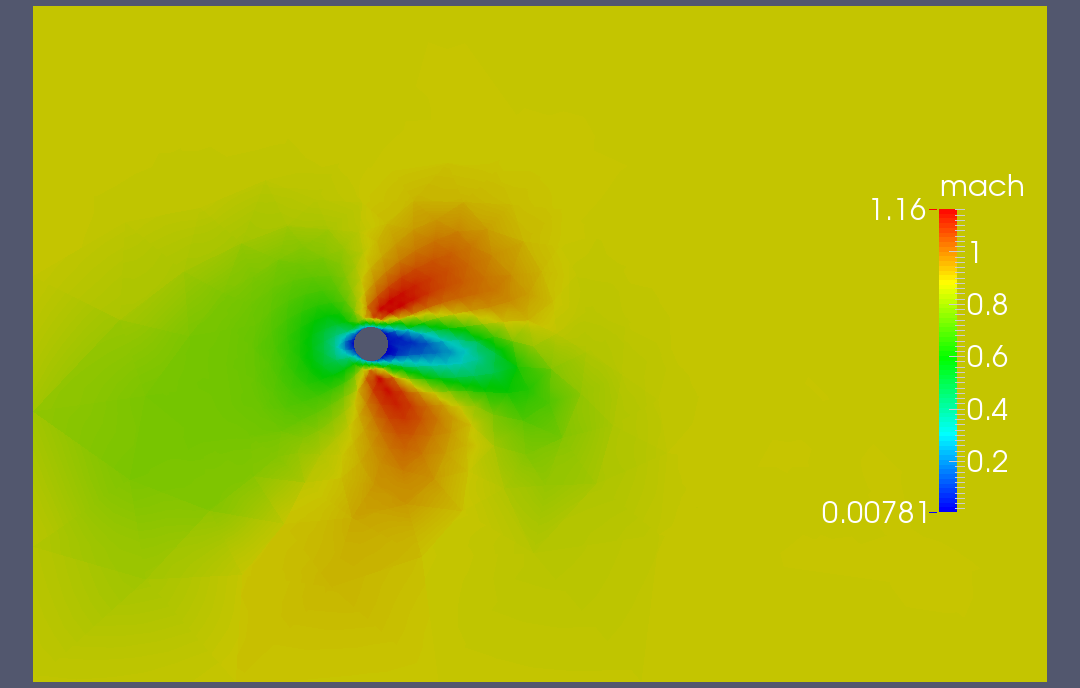
\includegraphics[width=0.55\textwidth]{figs/Ma0_87--Re1e6_Ma.png}
}
\hfill
\subfloat[Close-up view \label{fig:Ma0_87Re1e6_Ma__unstable_close}]{%
\centering
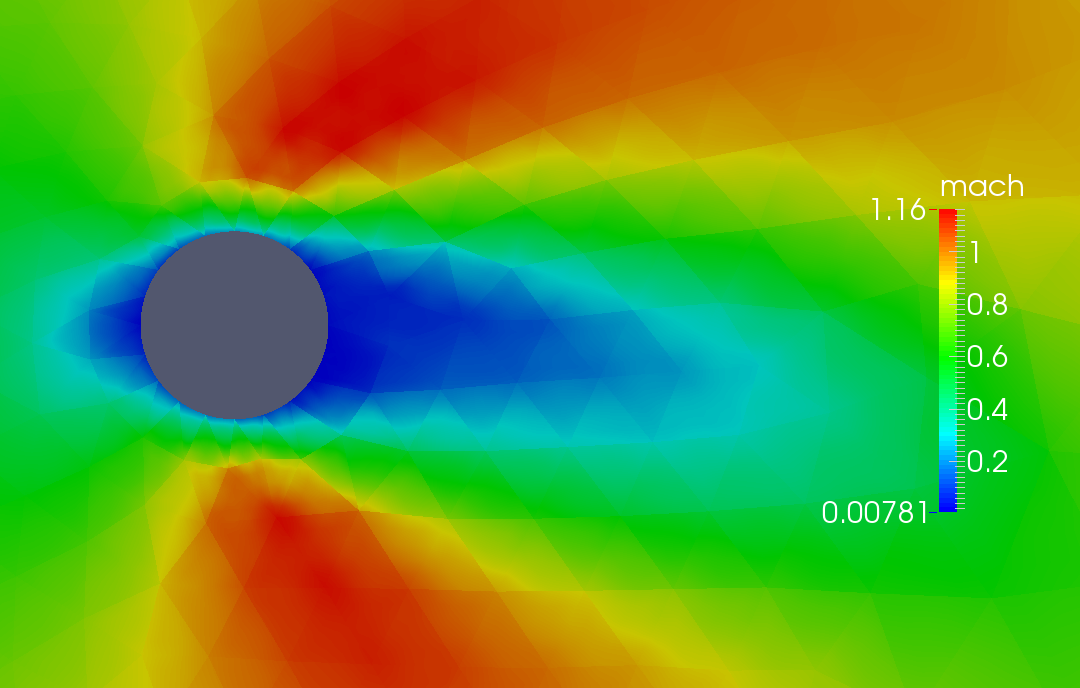
\includegraphics[width=0.55\textwidth]{figs/Ma0_87--Re1e6_Ma_closeup.png}
}

\hspace{-1cm}
\subfloat[Close-up view \label{fig:Ma0_87Re1e6_P__unstable}]{%
\centering
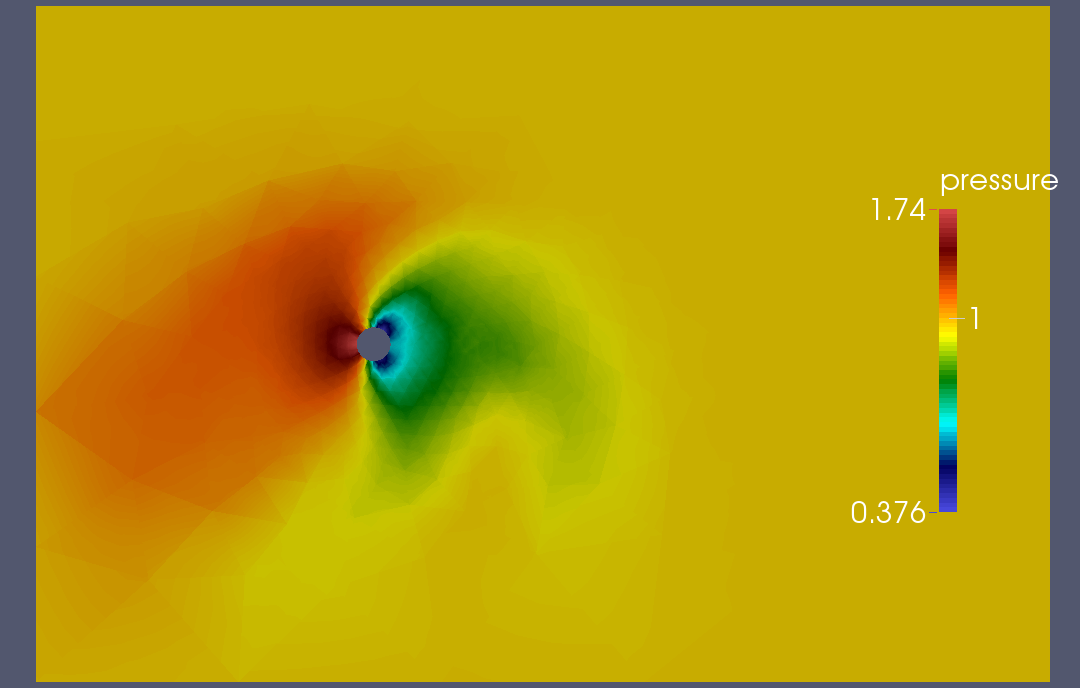
\includegraphics[width=0.55\textwidth]{figs/Ma0_87--Re1e6_P.png}
}
\hfill
\subfloat[Close-up view \label{fig:Ma0_87Re1e6_P__unstable_close}]{%
\centering
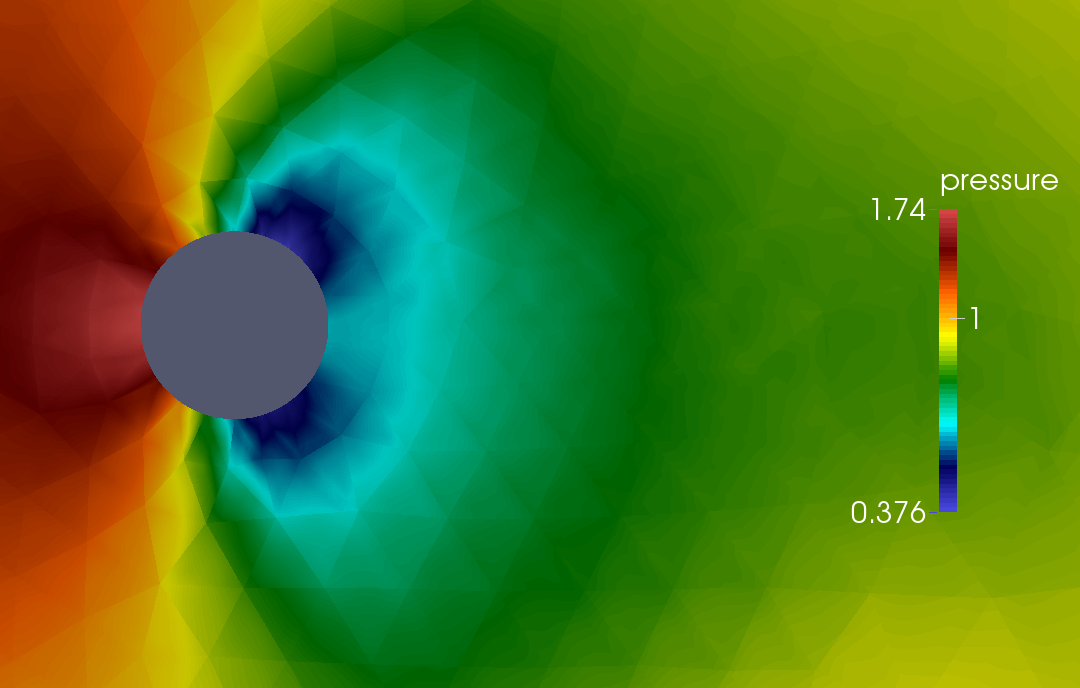
\includegraphics[width=0.55\textwidth]{figs/Ma0_87--Re1e6_P_closeup.png}
}
\caption{$\Re = 1e6, \Ma = 0.87, p = 4$}
\label{fig:Ma0.87Re1e6_unstable_Ma}
\end{figure*}